\section{Plan de d\'eveloppement}
\label{sec:plan:devt}



La premi�re partie est de consuitre les topologies virtualis�es et de
tester les performances de MTPCP en faisant varier les param�tres des
sous-flots. La seconde partie est de construire un alogrithme
d'ordonnancement r�pondant � des crit�res de s�curit�.
\vspace{0.5cm}

Les �tapes du d�veloppement suivront les points suivants:

\begin{itemize}
\item Pr�paration d'une machine mininet contenant MPTCP pour
  l'ensemble de l'�quipe.
\item Lecture et compr�hension du code de MPTCP et �criture de
  commentaires.
\item Pr�paration de plusieurs topologies : \emph{fat tree} pour
  simuler un \emph{data center} et d'une topologie permettant de
  tester la concurrence entre MPTCP et TCP.
\item Pr�paration d'une biblioth�que de tests et de mesures via l'API python
\item Pr�paration et �criture des algorithmes d'ordonnancement
\item Mesures de performances sur les diff�rents algorithmes
\end{itemize}




\begin{figure}[!htb]
  \begin{changemargin}{-2.0cm}{0.5cm}
    \centering
    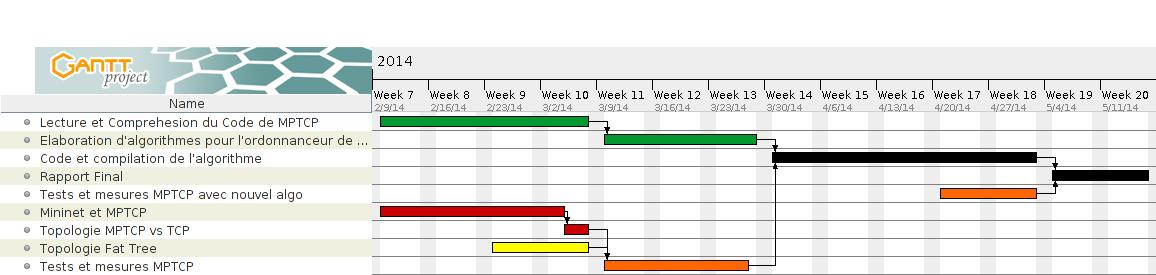
\includegraphics[width=1.2\textwidth]{../gantt/gant.jpg}
  \end{changemargin}
  \centering
  
  \caption{\textbf{Diagramme de Gantt}. Les couleurs correspondent �
    la r�partition grossi�re entre les membres de l'�quipe : en
    \emph{rouge} M. Ly, en \emph{jaune} M. Ravier et en \emph{vert}
    M. Dubois et M. Lam.}
  \label{fig:gantt}
  
\end{figure}

